             
%%%%%%%%%%%%%%%%%%%%%%%%%%%%%%%%%%%%%%%%%
% University Assignment Title Page 
% LaTeX Template
% Version 1.0 (27/12/12)
%
% This template has been downloaded from:
% http://www.LaTeXTemplates.com
%
% Original author:
% WikiBooks (http://en.wikibooks.org/wiki/LaTeX/Title_Creation)
%
% License:
% CC BY-NC-SA 3.0 (http://creativecommons.org/licenses/by-nc-sa/3.0/)
% 
% Instructions for using this template:
% This title page is capable of being compiled as is. This is not useful for 
% including it in another document. To do this, you have two options: 
%
% 1) Copy/paste everything between \begin{document} and \end{document} 
% starting at \begin{titlepage} and paste this into another LaTeX file where you 
% want your title page.
% OR
% 2) Remove everything outside the \begin{titlepage} and \end{titlepage} and 
% move this file to the same directory as the LaTeX file you wish to add it to. 
% Then add \input{./title_page_1.tex} to your LaTeX file where you want your
% title page.
%
%%%%%%%%%%%%%%%%%%%%%%%%%%%%%%%%%%%%%%%%%
%\title{Title page with logo}
%----------------------------------------------------------------------------------------
%   PACKAGES AND OTHER DOCUMENT CONFIGURATIONS
%----------------------------------------------------------------------------------------

\documentclass[12pt]{article}
\usepackage[english]{babel}
\usepackage[utf8x]{inputenc}
\usepackage{amsmath}
\usepackage{graphicx}
\usepackage[colorinlistoftodos]{todonotes}
\usepackage{setspace}

\usepackage{amssymb}
\usepackage{enumerate}
\usepackage[english]{babel}
\usepackage{caption}

\usepackage{listings}
\usepackage{color}
\usepackage[left=1.5cm, right=1.5cm, top=1.5cm, bottom=2cm]{geometry}
\usepackage{float}
\usepackage{subcaption}
\usepackage[toc,page]{appendix}
\setlength\parindent{0pt}
\usepackage{subcaption}

\bibliographystyle{ieeetr}  

\definecolor{codegreen}{rgb}{0,0.6,0}
\definecolor{codegray}{rgb}{0.5,0.5,0.5}
\definecolor{codepurple}{rgb}{0.58,0,0.82}
\definecolor{backcolour}{rgb}{0.95,0.95,0.92}

\lstdefinestyle{mystyle}{
	backgroundcolor=\color{backcolour},   
	commentstyle=\color{codegreen},
	keywordstyle=\color{magenta},
	numberstyle=\tiny\color{codegray},
	stringstyle=\color{codepurple},
	basicstyle=\footnotesize,
	breakatwhitespace=false,         
	breaklines=true,                 
	captionpos=b,                    
	keepspaces=true,                 
	numbers=left,                    
	numbersep=5pt,                  
	showspaces=false,                
	showstringspaces=false,
	showtabs=false,                  
	tabsize=2
}

\lstset{style=mystyle}

\begin{document}
	
\doublespacing

\begin{titlepage}

\newcommand{\HRule}{\rule{\linewidth}{0.5mm}} % Defines a new command for the horizontal lines, change thickness here

\center % Center everything on the page
 
%----------------------------------------------------------------------------------------
%   HEADING SECTIONS
%----------------------------------------------------------------------------------------

\textsc{\LARGE University of Melbourne}\\[1.5cm] % Name of your university/college
\textsc{\Large SWEN90004}\\[0.5cm] % Major heading such as course name
\textsc{\large Modelling Complex Software Systems}\\[0.5cm] % Minor heading such as course title

%----------------------------------------------------------------------------------------
%   TITLE SECTION
%----------------------------------------------------------------------------------------

\HRule \\[0.4cm]
{ \huge \bfseries Research Project}\\[0.4cm] % Title of your document
\HRule \\[1.5cm]

%----------------------------------------------------------------------------------------
%   AUTHOR SECTION
%----------------------------------------------------------------------------------------

\begin{minipage}{0.4\textwidth}
	\bfseries Group number : 47\\
	\bfseries Group member : Kaixiang Ren, Yang Zhang\\
	\bfseries Student ID : 956835
\end{minipage}\\[2cm]

% If you don't want a supervisor, uncomment the two lines below and remove the section above
%\Large \emph{Author:}\\
%John \textsc{Smith}\\[3cm] % Your name

%----------------------------------------------------------------------------------------
%   DATE SECTION
%----------------------------------------------------------------------------------------

{\large \today}\\[2cm] % Date, change the \today to a set date if you want to be precise

%----------------------------------------------------------------------------------------
%   LOGO SECTION
%----------------------------------------------------------------------------------------


\includegraphics[scale = 0.27]{logo.png}\\[1cm] % Include a department/university logo - this will require the graphicx package
 
%----------------------------------------------------------------------------------------

\vfill % Fill the rest of the page with whitespace

\end{titlepage}


\section{Background}
Wealth is always a  trade. Wealth distribution becomes an extremely hot topic for a long time, which contains two directions. The first direction focuses on how to increase the wealth gap between the poor and the rich. The second direction mainly ana how to 
\section{Design}
\subsection{Original Model}
\subsection{Extensions}

\section{Results}
\section{Discussion}







\newpage
\section{Introduction}

With the price dropdown of storage unit, a modern main memory database can potentially store itself entirely within the main memory, which leads to faster computing and transactions\cite{garcia1992main}.

However, it also means the concurrency control transfers its duty from being able to serve other transactions when current one is stall due to the lack of accessing speed towards handling transactions contention on single resource. When different transactions happen concurrently and they all try to access the same data resource, the contention could happen.

In general, when two transactions try to read the same data out of database, there would be no damage done to the transaction integrity\cite{gray1992transaction}. However, in most contexts, transactions try to write to the data resource, which may leads to different scenarios:
\begin{itemize}
\item Dirty Read: where a transaction is allowed to read some not yet committed write from other transactions.

\item Lost Updates: where a transaction read in other's committed write, but later on that committed write gets rolled back.

\item Non-repeatable reads: where a transaction read the same row twice but due to others write, the value changes.

\item Phantom reads: where a transaction received the recordings but some added or removed rows by other transactions were not included.
\end{itemize}


Isolation levels are defined correspondingly, it states how the integrity of the transactions shall be handled by blocking out the resources. Despite different database management system implements the isolation levels differently, some basic levels exist among most of them:
\begin{itemize}
	\item Serilizable: it requires multiple transaction could be serialized and comes out in the same result which is the highest isolation level.
	
	\item Repeatable reads: it requires the transaction must be avoid unrepeatable read.
	
	\item Read committed: it allows transaction to read others' writes as long as they are committed.
	
	\item Read uncommitted: it gives transaction most freedom on accessing the resources which is the lowest isolation level.
\end{itemize}


Commonly when a contention occurs, we would like one transaction locks down the resource it wants, so that transaction can hold locks inferring what types of operation it would do to the data, either Read or Write. Multiple transactions can only access the same data when all of them want to read the data. All the lock based concurrency control protocols can be categorized into pessimistic where each transaction assume the contention would happen, so it requires lock to the resource; the other type of concurrency control is optimistic, where each transaction consider the resource would always be available to itself, so it access as usual until a contention happens, then based on different protocols, one of the competing transaction shall roll back.
\section{Literature review}

In the process of our research, we have tried out several databases in real life setup. And beyond the concurrency controls, we have found that not all of the databases implement isolation levels the same\cite{adya2000generalized}, and tested MySQL and PostgreSQL on this fact. It is cleared that not all databases setup the isolation levels as they claimed to be due to the fact that with minimum amount of isolation, the transactions would face abort and roll back frequently, which is not ideal. To realize the isolation level design, different databases use different concurrency control protocols. Modern databases mostly adapted four types of concurrency control protocols:

Two-Phase Locking: for transactions, there would be a lock growing phase when resources got locked and no locks can be released, so that others cannot work with it, and there would be a shrinking phase where locks are released and no locks are acquired.

Multiple Version Concurrency Control: it normally uses a typical type of isolation level called ``snapshot isolation" which means when a transaction want to write to a resource, it would take a snapshot of that resource, and privately working on that snapshot hence it would not block any future read on this resource\cite{berenson1995critique}.

Optimistic Concurrency Control: it is a protocol under Timestamp Ordering Concurrency Control, containing three phases set for the each transaction, it can read, validation, and commit. While expecting no confliction, each transaction would read, which consists of both read and write means operating on data, validate whether commit is viable, if yes, then commit, otherwise rollback.

Timestamp Ordering Concurrency Control: it is a class of concurrency control protocols, which includes Optimistic Concurrency Control protocols, but it also represents a protocol using timestamp to making decision on which transaction shall rollback. By using this concurrency control, it gives each transaction a timestamp when it starts, and when two transactions compete on one resource, the old one should always abort when the newer transaction has already in use with the resource.

All of these four concurrency control protocols are basics of modern database concurrency control, many variations emerged to satisfiy different needs and improve the performance. Such as, researchers have purposed a balanced concurrency control to reduce false abort by utilize the dependencies of data in comparison to optimistic concurrency control\cite{yuan2016bcc}; and people have also done extensive research in improving MVCC, for example, researchers have purposed using in-place update and before-image version storage to reduce the overhead of MVCC hence improve the performance\cite{neumann2015fast}; there are also improvements done to timestamp ordering, which researchers purposed a time travel algorithm based on time ordering concurrency control, it aims to solve On-line Transaction Processing problems\cite{yu2016tictoc}.

Beyond the research we have done, we also look into some possible changes could be made to Timestamp Ordering protocol. We suggest in extreme case of a nearly finished transaction has competition against just started transaction, the old transaction should not rollback, but rather letting the new transaction rollback so minimum amount of time and computing is wasted. And also, transaction shall gain priority based on the time they have been executed and the estimated time that it could be finished, hence abort decision could be better made to avoid wastes.

\section{Multi-version Concurrency Control(MVCC)}
\subsection{Basic Idea \& History}
As we talked above, there are multiple ways to deal with conflicts in concurrency control theory. Optimistically, we assume there is not conflict and deal with it if it actually happens. Pessimistically, we could apply locking mechanisms to avoid or deal with every possible conflict. The most famous methods are Read/Write locks and Two-Phase lock. The lock mechanism could perfectly solve different types of conflicts. Rollback is a time-consuming operation, which is not suitable for high concurrent environment. However, similar to other programming language, the lock always leads to performance issue because locks tend to result in contention and severe contention will significantly impact the scalability, which contradict the purpose of concurrency.\\

Back to the concept of conflict, we could conclude the conflict into read-write conflict and write-write conflict. The idea of \textbf{Multi-version Concurrency Control} is to solve the read-write conflict and get rid of most of lock operations at the same time. The method is to create a snapshot when transaction begins or query begins based on different isolation level, which is also called \textbf{Snapshot Isolation}. The consequence of MVCC should be :
\begin{itemize}
	\item Readers don't block writers
	\item Writers don't block readers
\end{itemize}
//TODO: References\\
 \textbf{Multi-version Concurrency Control} was first proposed by David P. Reed's paper in 1978. Then in 1981, the paper "Concurrency Control in Distributed Database Systems" by Phil Bernstein and Nathan Goodman clearly and detailedly analyzed and expounded the MVCC comparing to other basic synchronization techniques \cite{Bernstein1981}. Then the MVCC was first implemented by Rdb/VMS and InterBase at DEC in early 1980s \cite{Bernstein1983}. Both of implementations were designed by Jim Starkey.

\subsection{Implementation}
The implementations of MVCC are various and there is not a standard till now, which results from no limitation of implementation detail. The differences mainly lay in four aspects.
\begin{itemize}
	\item Concurrency Control Protocol
	\item Version Storage
	\item Garbage Collection
	\item Index Management
\end{itemize}
Here we will introduce the MVCC mechanisms and its related four aspects when implementing the \textbf{Multi-version Concurrency Control}.
\subsubsection{MVCC Mechanism}
Before diving into MVCC mechanism, we need to introduce the common metadata used in MVCC implementation. \\

As we need to store values with multiple versions, there should be some metadata to assist us manipulating and controlling different versions. Common idea is that two extra attributes are attached to original database and one extra table to record status of every records. We list most common four metadata attributes of a version tuple (Txn stands for transaction).
\begin{itemize}
	\item TxnId: Responsible transaction id for current record.
	\item Begin: Timestamps or transaction that created this version record.
	\item End: Timestamps or transaction that updates this version record. BEGIN-TS and END-TS construct the version lifetime together.
	\item Status: The status of every version, typically there are only two status, committed and active.
\end{itemize}
Here we show the example tables and two example transactions to demonstrate the whole process of MVCC.

\begin{table}
	\parbox{.45\linewidth}{
		\centering
		\begin{tabular}{|c|c|c|c|}
			\hline
			version&Value&Begin&End\\\hline
			$A_0$&1234&0& \\\hline
			&&&\\\hline
			&&&\\\hline
		\end{tabular}
		\caption*{Database Table}
	}
	\hfill
	\parbox{.45\linewidth}{
		\begin{tabular}{|c|c|c|}
			\hline
			TxnId&Timestamps&Status\\\hline
			$T_1$&1&active \\\hline
			&&\\\hline
			&&\\\hline
		\end{tabular}
		\caption*{Txn Status Table}
	}
\caption{Example Tables\label{table1}}
\end{table}

Firstly, we will talk about the visibility of version table. There are three conditions, transaction ID, timestamps and isolation level. As the transaction IDs  are incrementing, we could firstly use transaction ID to judge the sequence of transactions. There are generally three rules to decide whether a transaction can see the target version.	
\begin{itemize}
	\item If current transaction ID is larger than the id that inserted this record, it's allowed to read the target version record.
	\item If current transaction ID is lower than the id that inserted this record, the timestamps needs to be considered based on different isolation level.
	\begin{itemize}
		\item For \textbf{READ COMMITTED}, the timestamps of currently executing statement will decide whether version record is visible.
		\item As for \textbf{REPEATABLE READ} or \textbf{SERIALIZABLE}, all the read operations of current transaction relies on the timestamps when it starts.
	\end{itemize}
\end{itemize}

For clearer explanation, we provide a concrete updating process to demonstrate how this table gets modified. Here is the general flow chart for example. The Isolation level in this example is \textbf{READ COMMITTED}.
\begin{figure}[H]
	\centering
	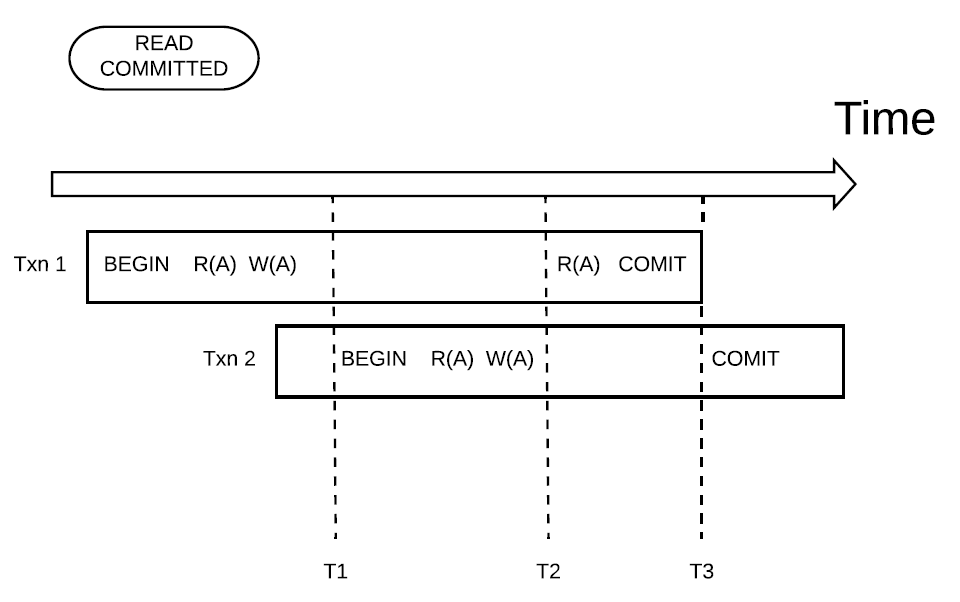
\includegraphics[scale=0.36]{demo1.png}
\end{figure}
When transaction 1 begins and reads the data, tables should look like Table \ref{table1}. After transaction 1 write new data for record A, a new version of record A will be created inside the transaction. Tables should look like following tables.
\begin{table}[H]
	\parbox{.45\linewidth}{
		\centering
		\begin{tabular}{|c|c|c|c|}
			\hline
			version&Value&Begin&End\\\hline
			$A_0$&123&0&1 \\\hline
			$A_1$&456&1& \\\hline
			&&&\\\hline
		\end{tabular}
		\caption*{Database Table}
	}
	\hfill
	\parbox{.45\linewidth}{
		\begin{tabular}{|c|c|c|}
			\hline
			TxnId&Timestamps&Status\\\hline
			$T_1$&1&active \\\hline
			&&\\\hline
			&&\\\hline
		\end{tabular}
		\caption*{Txn Status Table}
	}
	\caption{First Updated Tables\label{table2}}
\end{table}
At the same time, transaction 2 begins and reads the data. It can not know the modification at present and the data transaction 2 read is the same as Table \ref{table1} as well. Then when transaction 2 attempts to write new data for record A, It senses that there is another transaction currently modifying the data. It needs to wait for transaction 1 commits in order to avoid write-write conflict.\\

As time goes, transaction 1 read the tables, whose values and versions should be the same as Table \ref{table2}. Then it commits and transaction status table records at the same time. Now, the transaction 2 start writing and database table gets updated. The tables should be as following.
\begin{table}[H]
	\parbox{.45\linewidth}{
		\centering
		\begin{tabular}{|c|c|c|c|}
			\hline
			version&Value&Begin&End\\\hline
			$A_0$&123&0&1 \\\hline
			$A_1$&456&1&2 \\\hline
			$A_2$&789&2& \\\hline
		\end{tabular}
		\caption*{Database Table}
	}
	\hfill
	\parbox{.45\linewidth}{
		\begin{tabular}{|c|c|c|}
			\hline
			TxnId&Timestamps&Status\\\hline
			$T_1$&1&committed \\\hline
			$T_1$&2&active \\\hline
			&&\\\hline
		\end{tabular}
		\caption*{Txn Status Table}
	}
	\caption{Second Updated Tables\label{table3}}
\end{table}
This is the whole process of \textbf{Multi-version Concurrency Control}. The next part is to evaluate four detailed aspects when implementing it. 

\subsubsection{Concurrency Control Protocol}
MVCC is designed to manipulate read-write conflict. However, we need another concurrency control protocol to deal with write-write conflict. They are the same as we talked in previous sections, timestamps ordering, 2-phase locking and optimistic concurrency control. Therefore, protocols of MVCC could be summarized into three types.
\begin{itemize}
	\item MV-2PL
	\item MV-TO
	\item MV-OCC
\end{itemize} 
Concurrency control protocol ensures the consistency and visibility in concurrent access environment. Back to our previous example, we actually applied MV-2PL because we assume following write operations need to wait for earlier write operations. It's actually lock mechanism. As for MV-TO, the serial order will rely on timestamps of transactions. MV-OCC similarly obeys its three-phase protocol to keep consistency.\\
 
\subsubsection{Version Storage}
As multiple versions of record created, there should be a method to store all the versions. Due to lock of standard, different database service providers apply various version storage strategies. In general, there are three different storage methods.
\begin{itemize}
	\item Append-Only Storage: The method aims to store different versions of records in the same table. This is the simplest way to store the versions. There should be a pointer to connect all the versions of a record together. In previous example, we applied this method. Furthermore, there are two directions when connecting versions.
	\begin{itemize}
		\item Oldest-to-Newest(O2N)
		\item Newest-to-Oldest(N2O)
	\end{itemize}
	\item Time-Travel Storage: The basic idea of this method is to create a new table to store all out-of-date versions while latest version is stored in database table. Whenever there is update, current version will be moved into Time-travel table while new version will overwrite original one in main database table. Database table and time-travel table are connected by pointers. Inside of time-travel table, both directions could be selected. This strategy is typically used in bank database system, which means every information of old version needs to be stored for possible check in the future. 
	\item Delta Storage: Similar to Time-Travel Storage, there will be a new table to store old versions and main database table points to this new table. The difference is that only the value of every version is stored in delta table. database table's Pointer always points to newest version in delta table. Transaction could recreate old version for rollback by simply applying the reversed delta. 
\end{itemize}
\subsubsection{Garbage Collection}
As transactions executed one by one, there will always be some versions that will not and can not be visible any more. The garbage collection mechanism could start from two levels. The system could check every version tuple to find out order and unused version tuples and remove them. The other idea is based on expired transaction. DBMS determines the visibility of version tuples created by one transaction when this transaction is finished. The version tuples that are no longer visible will be removed. There are two methods to implement tuple-level garbage collection. 
\begin{itemize}
	\item Tuple Level
		\begin{itemize}
			\item Background Vacuuming: require an extra thread to check and remove all reclaimable versions periodically. 
			
			\item Cooperative Cleaning: don't need extra thread. When worker thread traverses the version chain. It will check the visibility of versions. If there is any reclaimable version, worker thread will remove it and update the pointer to oldest visible version. However, there is a primary requirement in this mode. Only Oldest-to-Newest version chain is permitted because the other version chain mode will not traverse to oldest version tuple.  
		\end{itemize}
	\item Transaction Level
\end{itemize}
As our previous example shows, there is a table called Txn Status Table and we assume the size of table is fixed. In transaction level situation, new transaction will be assigned into the table. The transaction-level garbage collection starts when the Txn Status Table is full and all transactions in it are committed. In this way, the garbage collection needs to track the status of Txn Status Table, which may impair the performance.    
\subsubsection{Index Management}
//TODO: Reference\\
The final part is related to pointer we mentioned multiple times above. Primary key always connects to the head of version table. Whenever a new version is inserted, the pointer will be updated to new head of version table. However, this is not a good solution for secondary keys. If they connects to the head of version table physically. Every time update happens, all pointers of secondary keys need to be updated. The alternative solution is logical pointer. 

\begin{itemize}
	\item Logical Pointer
	\item Physical Pointer
\end{itemize}
There are two ways to implement the logical pointer. Firstly, secondary keys could directly connects to primary keys. The values of secondary keys will be automatically updated whenever value of primary key updates. MySQL does this way. Another way is to build a middle layer to map the physical address and multiple secondary keys. Whenever new version is created, system will only update the value inside of middle layer. Generally speaking, the performance of logical index will be improved about 25\% to 40\%.\\

Finally, here we list the configurations of multiple database service providers.
\begin{table}[H]
	\scalebox{0.8}{
		\begin{tabular}{c | c c c c}
			&Protocol&Version Storage&GC&Indexes\\\hline
			Oracle& MV-2PL&Delta&Vacuum&Logical\\
			Postgres&MV-2PL/MV-TO&Append-Only&Vacuum&Physical\\
			MySQL-InnoDB&MV-2PL&Delta&Vacuum&Logical\\
			HYRISE&MV-OCC&Append-Only&-&Physical\\
			Hekaton&MV-OCC&Append-Only&Cooperative&Physical\\
			MemSQL&MV-OCC&Append-Only&Vacuum&Physical\\
			SAP HAHA&MV-2PL&Time-travel&Hybrid&Logical\\
			NuoDB&MV-2PL&Append-Only&Vacuum&Logical\\
			HyPer&MV-OCC&Delta&Transaction Level&Logical\\
		\end{tabular}
	}
		
\end{table}
\section{Timestamp Ordering Concurrency Control}

Timestamp ordering is an old concurrency control model dated back to 1980s\cite{li1987performance}. It is classified as an Optimistic Concurrency Control protocol which means it does not assume a contention would occur, therefore no locking mechanisms are implemented in this algorithm.

\subsection{Basic Timestamp Ordering}
Timestamp Ordering has a basic idea of older transaction should not compete with newer transaction. It is done by assigning each transaction a timestamp, the timestamp would be assigned after the transaction starts executing, it could be either at the start of a transaction or at the commit of a transaction, or even having timestamp for both start and commit.

Basic Timestamp Ordering algorithm assigns timestamp whenever a transaction starts, it gives each object a read timestamp and a write timestamp to record the time of latest transaction which has used this object. And when a transaction wants to read an object, it has to make sure the object has not be written by any other transaction from ``future'' which means it's timestamp shall not be smaller than the object's write timestamp, otherwise this transaction shall rollback to be assigned with new timestamp; similar with writing, only the transaction is allowed to write to an object when it is neither read or written by any ``future'' transaction.

\begin{figure}[H]
	\centering
	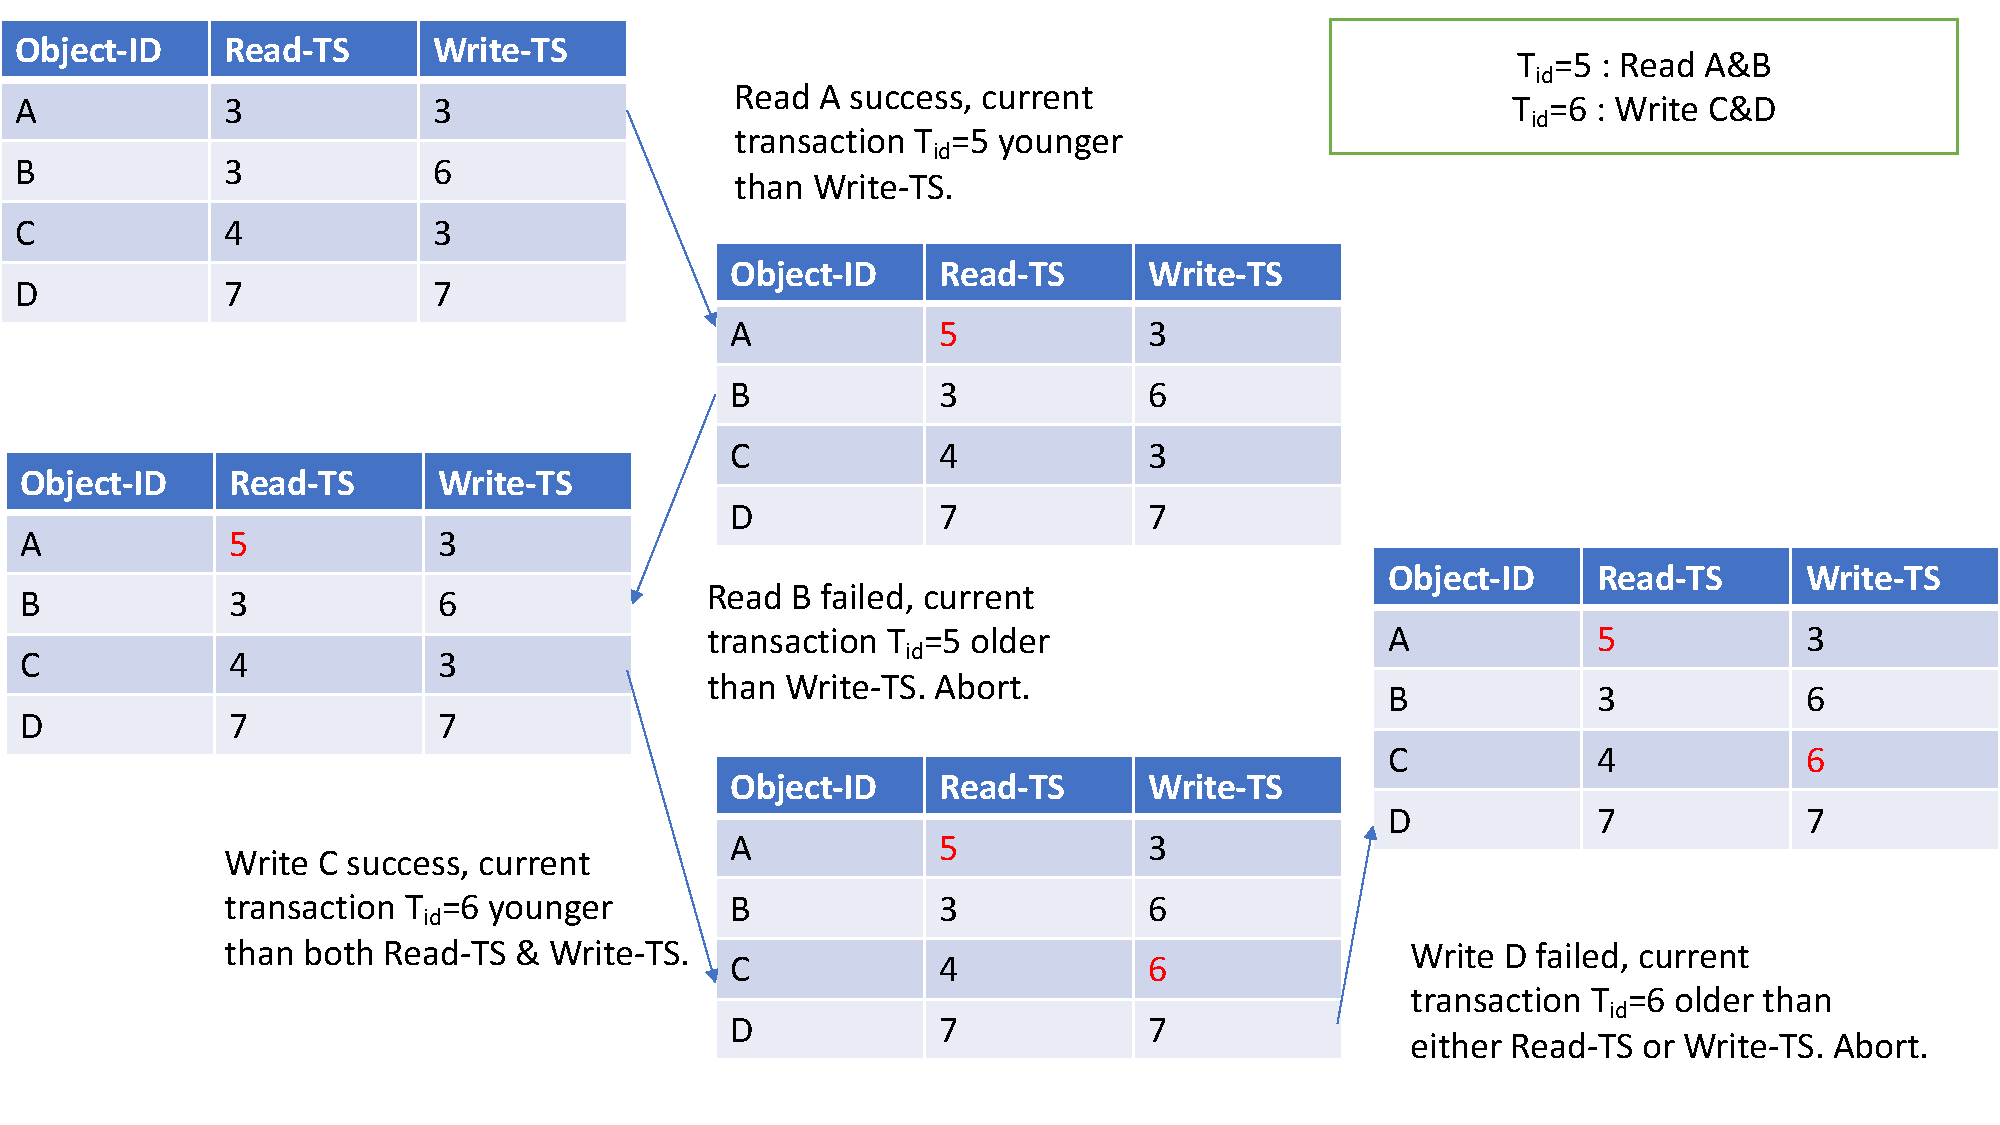
\includegraphics[width=0.8\linewidth]{basicTO.pdf}
	\caption{Basic Timestamp Ordering Example}	
\end{figure}

In general, this concurrency control requires no lock so it reduces the overhead of locking, however, there are few issues with it.

First, how to define the timestamp is crucial. Because timestamp must be able to uniquely identify each transaction, otherwise this algorithm is useless. And timestamp should never go back in time because it is not physically possible. Two types of timestamp are considered, one is using system clock, which could violates the second requirement whenever it comes to day light saving time, because time would go back for one hour; alternatively, a counter could be used, with the increasing number of transactions, counter could eventually wrap up, and it would go back to 1 indicating the time went backwards\cite{bernstein1980timestamp}. And in modern database systems, especially in distributed databases, it is very complicated to maintain a global clock ensures unique timestamp globally\cite{corbett2013spanner}.

Second, abort the transaction and rollback to restart cost a lot time and computing resources. And if a transaction is very long it would always be blocked by newer transactions so that it could never finish. Different variations are purposed to minimize the need for abort, most improvements are based on solving this issue.

Basic Timestamp Ordering doesn't have the best performance\cite{harding2017evaluation}, and due to the difficulty on actual timestamp generation, it is not very popular as concurrency control protocols in modern databases. However, it still plays a subtle rule in modern database design, and it's variants like multiple version timestamp ordering is very relevant to today's transaction concurrency control.
\subsection{Thomas Write Rule}

Thomas Write Rule is an improvement made to resolve the write-write conflict. The core philosophy is when a transaction tries to write to an object, and that object has already been written by a ``future'' transaction, this transaction would still do it's write in it's local version but not write to the global, because it knows whatever it writes would be overwritten by the ``future'' transaction.

\begin{figure}[H]
	\centering
	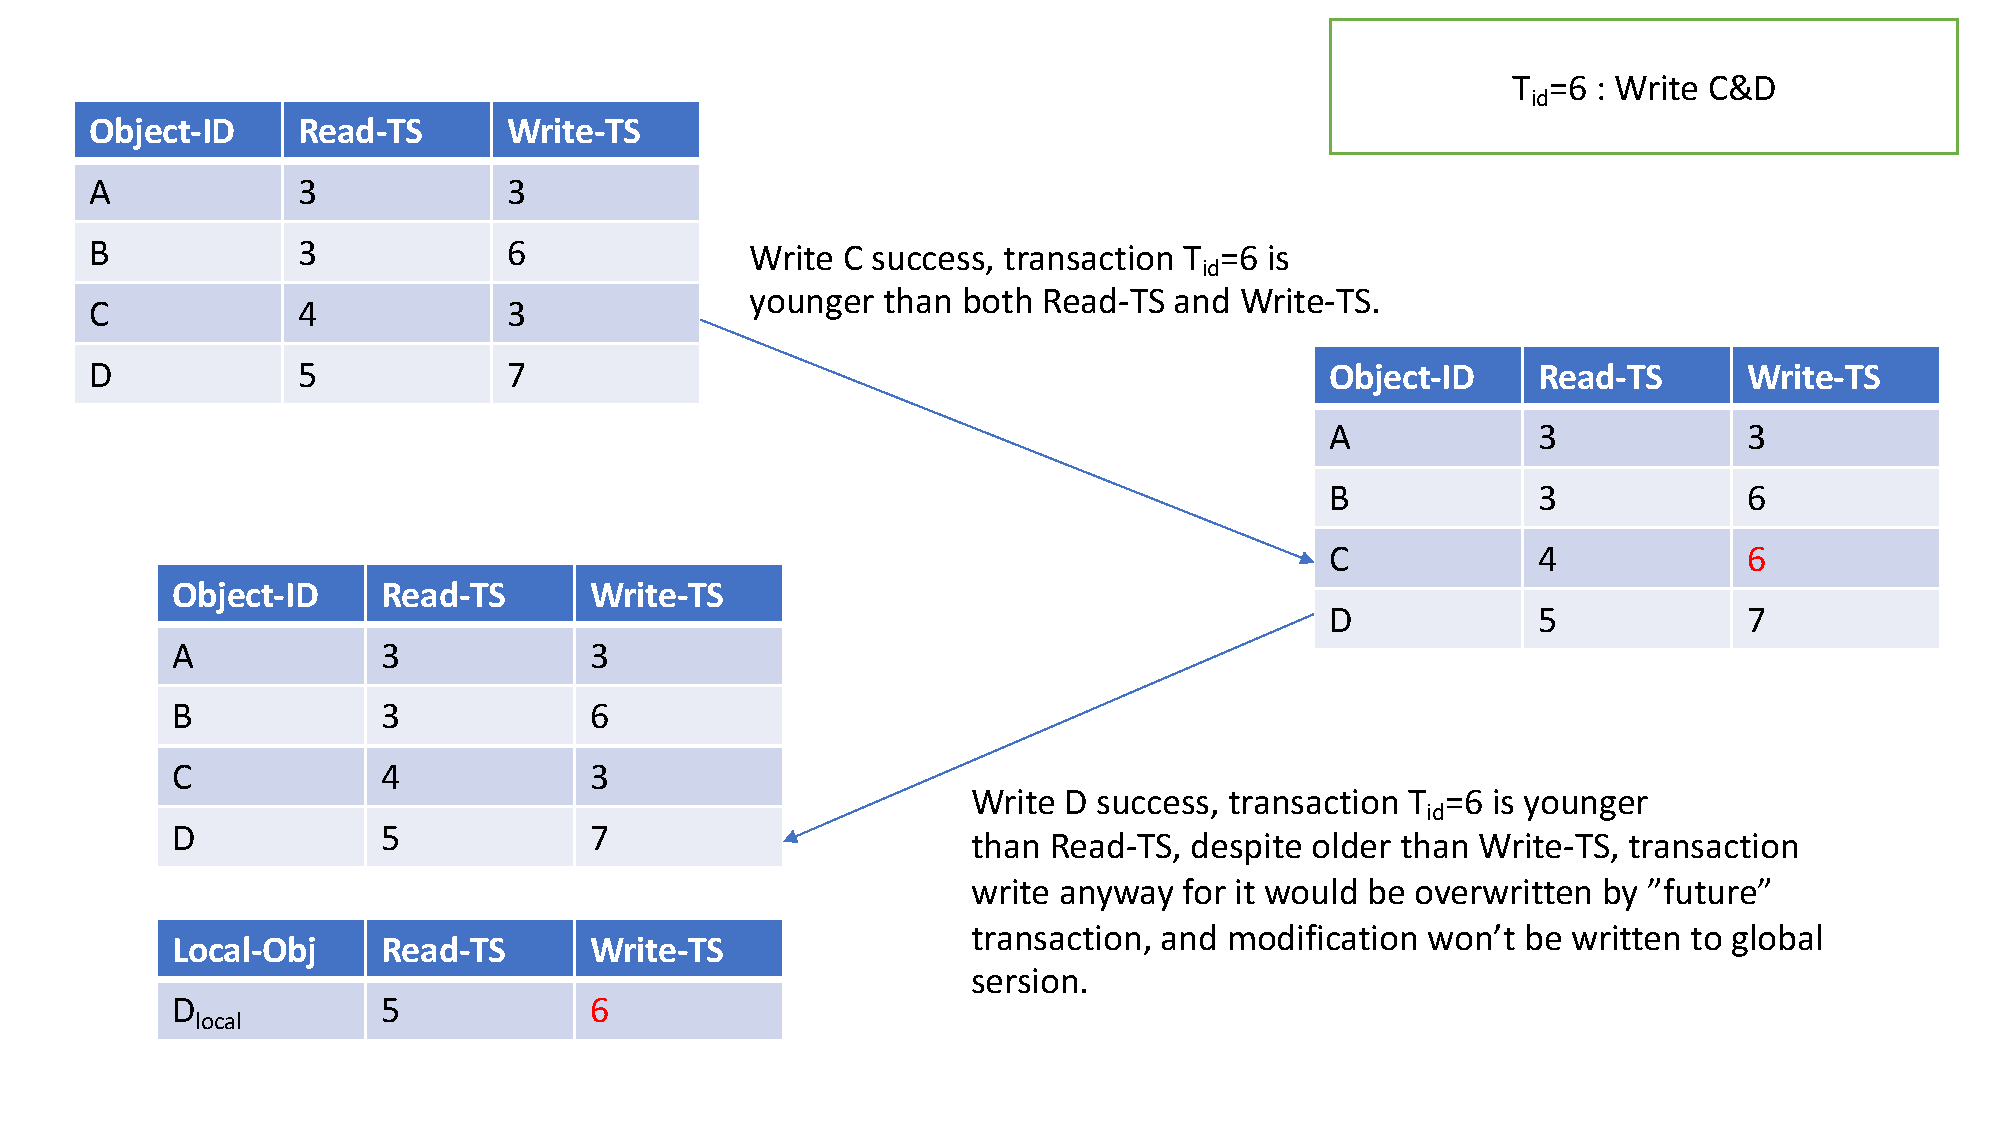
\includegraphics[width=0.8\linewidth]{twrTO.pdf}
	\caption{Thomas Write Rule Example}	
\end{figure}

It is a relatively simple improvement on timestamp ordering which resolve the abort and rollback issue over the write-write conflict. It could be effectively applied along with Multi-Version Concurrency Control such that it could handle this type of conflicts while MVCC cannot.

However, this strategy still has limits, the one we thought about is it ignores the possibility that other transactions need the ``older'' transaction's written value for their usage. In the case of transactions have dependencies on the data they write to a certain object, this strategy will break such dependency or at least other data pipeline shall be utilized. For example, if alice wants to transfer \$100 to bob, meanwhile bob withdraw \$50, for bob's account, two transaction one write +100 and the other write -50, if conflicts happened and handled using this rule, one of the data would be missing.

\subsection{Multiple Version Timestamp Ordering}

Multi-Version Timestamp Ordering is a example of one transaction has multiple timestamps\cite{reed1978naming}. It could be seen as the original version of Multi-Version Concurrency Control.

It requires each object/resource to maintain a current transaction id to show whether there is any transaction currently working on it; a read timestamp to show the latest read by a transaction; and a begin timestamp and end timestamp to show case when is this object get modified and whether it is the latest version of this object with infinity on end timestamp.

When a transaction wants to read an object, it would ensure that no other transaction is currently writing to it by see the transaction id equals 0, and it will check the begin timestamp and end timestamp making sure it falls within this time period, then it would read the object and update the read timestamp; when a transaction wants to write an object, it would also make sure no other transaction is writing to it, and it's timestamp falls within the begin and end timestamp of that object, then it would copy that object, giving a new physical record, and having lock on this logical record which means both old and new version has transaction id equals to the this transaction, then it would write to the object, remove the lock, and update the old version with end timestamp equals to this transaction's timestamp, the new transaction would start from this transaction timestamp and end in infinity to show it is the latest version. 

\begin{figure}[H]
	\centering
	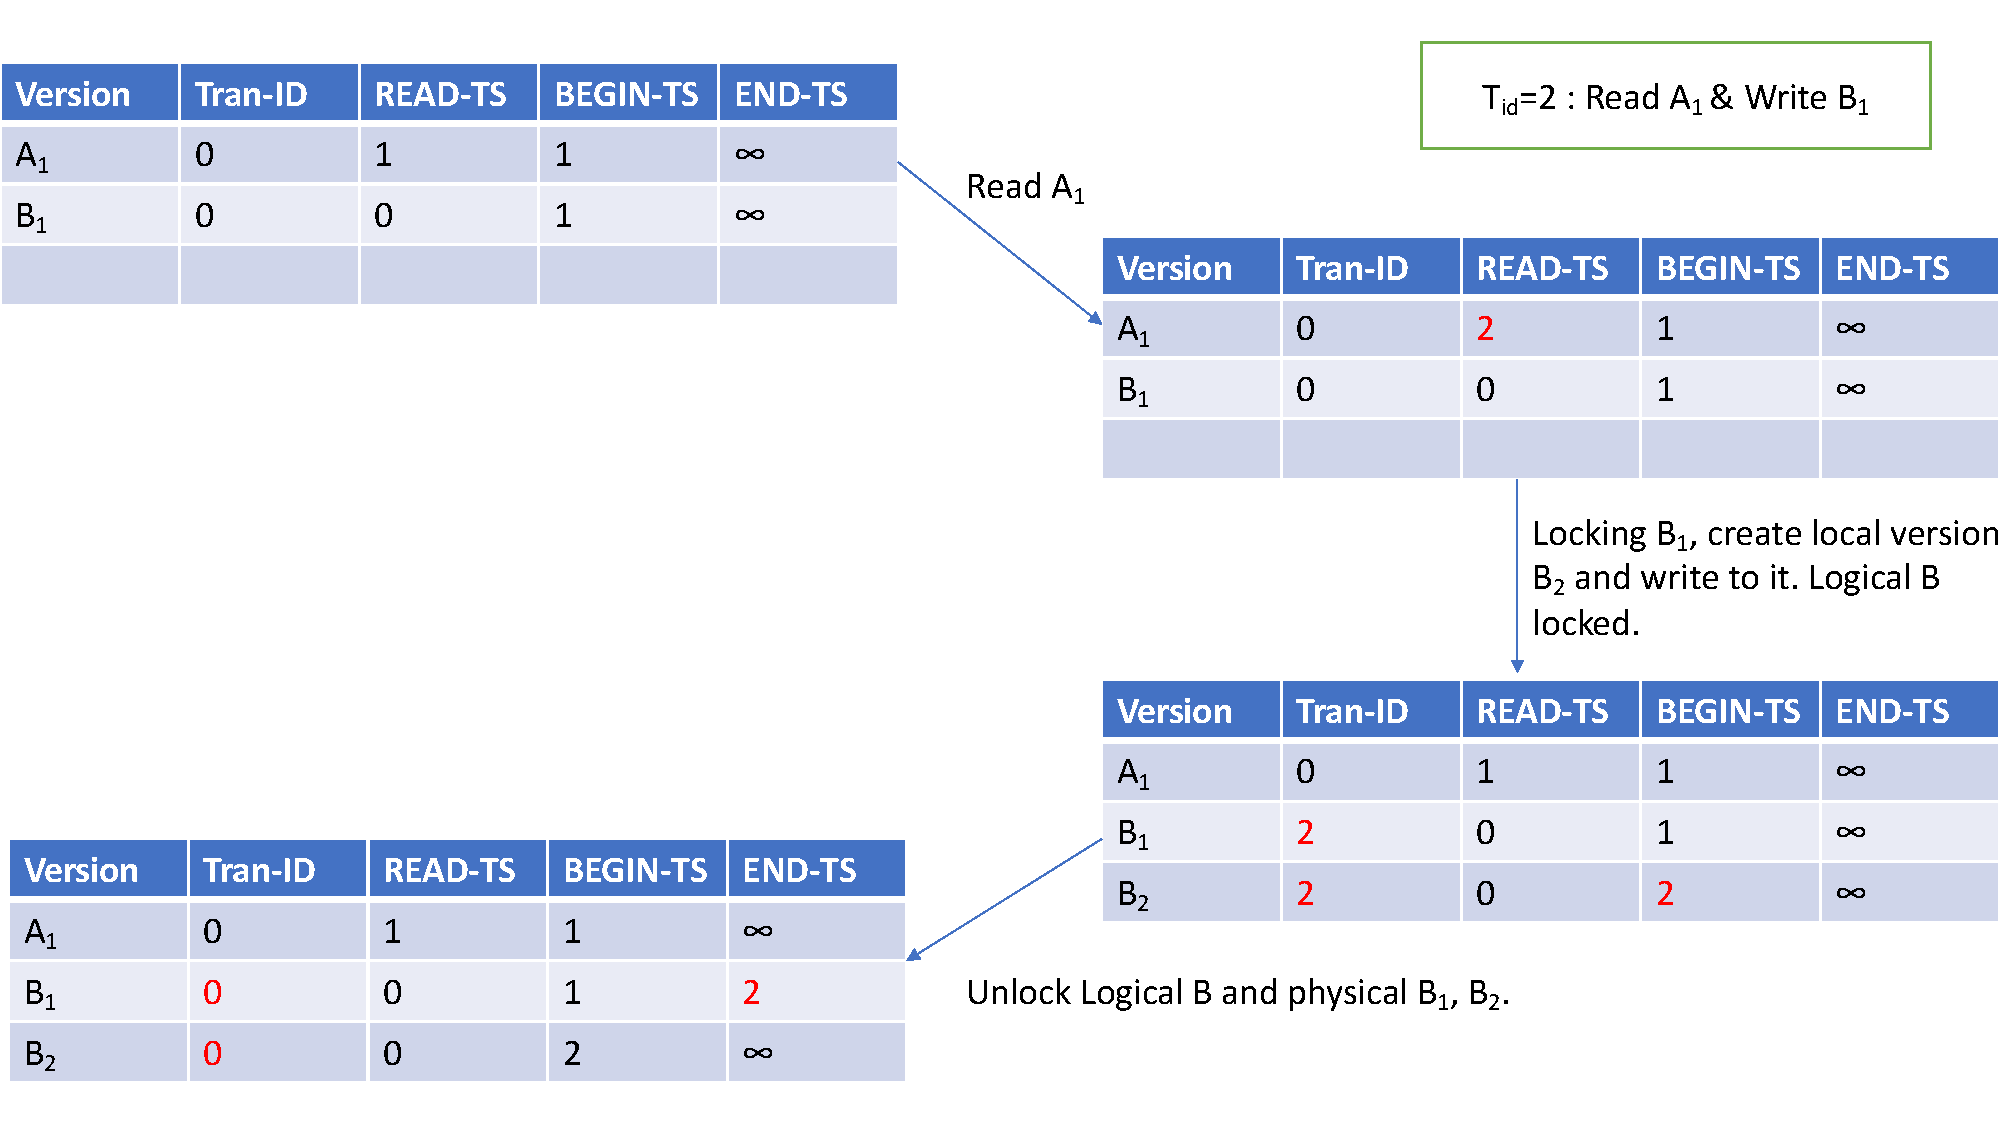
\includegraphics[width=0.9\linewidth]{MVTO.pdf}
	\caption{Multi-Version Timestamp Ordering Example}
\end{figure}

As evaluated by CMU researchers, MVTO has very good performance, and within this research, several benchmarks show Multi-Version Timestamp Ordering often have 40\% to 100\% performance improvement as compared to Multi-Version Two Phase Lock and Multi-Version Optimistic Concurrency Control\cite{wu2017empirical}. And from this research, it is shown that append-only versioning is the best way to increase the throughput by using multiple threads. And this protocol is proven to be very efficient in modern On-Line Transaction Processing tasks.

\subsection{Tictoc Algorithm}

A modern adaptation to timestamp ordering would be the Tictoc algorithm from researchers in MIT\cite{yu2016tictoc}. The major improvement of this algorithm is it does not require a centralized system to assign timestamp to each transaction, instead the timestamp is calculated when the transaction commits based on the read or write timestamp stored in data/tuple that relative to this transaction.

This algorithm requires each transaction maintains two sets of two timestamp for all object/resource it accessed. When a transaction read an object, it set to it's read set timestamp using the object's read and write timestamp, and when it write to an object, it copies the object's read and write timestamp, so when it finally making decision on it's own timestamp when facing commit, it would pick the larger one from the read set write timestamp and write set read timestamp plus one. It would also lock down the object it write to using similar technique to Optimistic Concurrency Control. Then if it's read object has not been written by others, it commits, otherwise, it would check whether it's timestamp is within that read object's read and write timestamp, and commit if yes.

\begin{figure}[H]
	\centering
	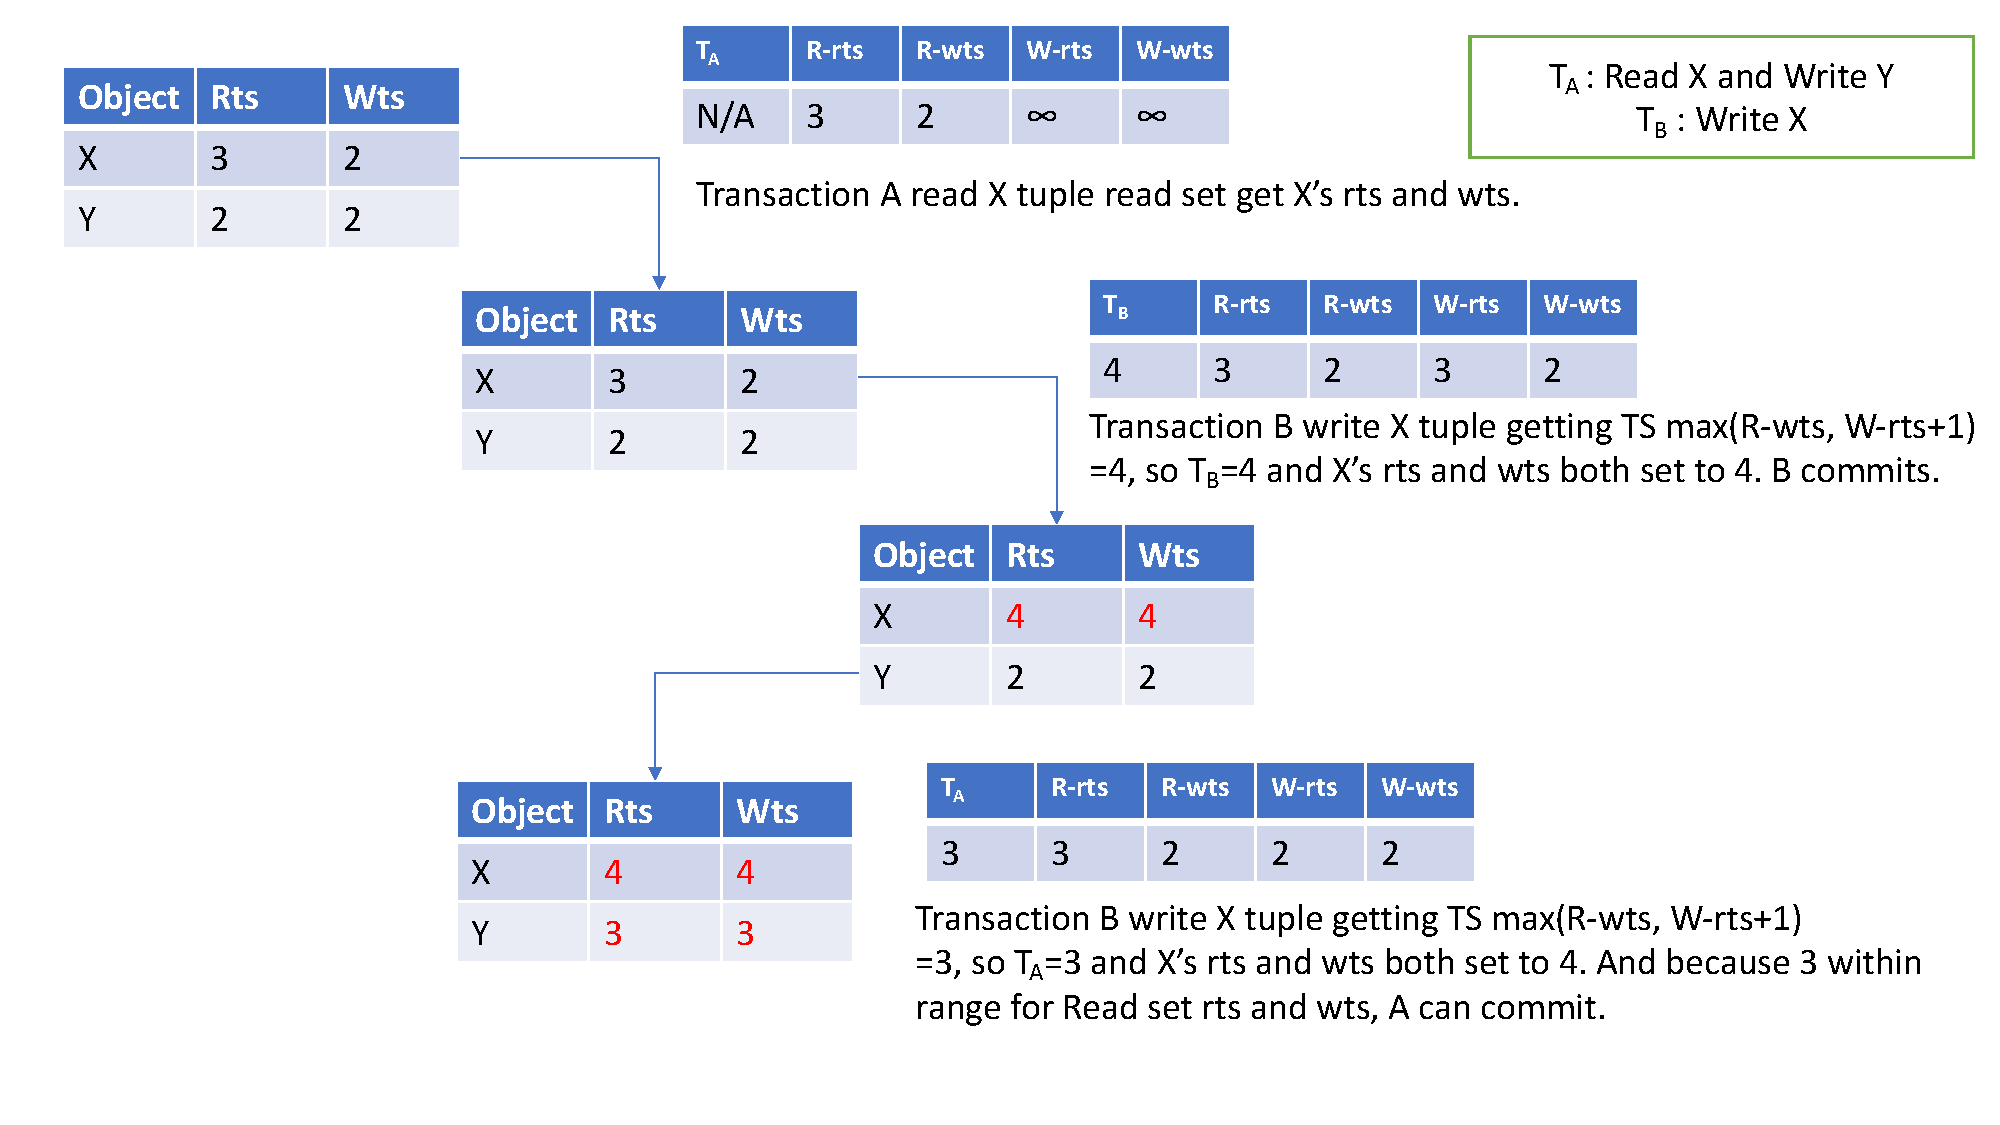
\includegraphics[width=0.9\linewidth]{tictocTO.pdf}
	\caption{Tictoc Timestamp Ordering Example}
\end{figure}

In the same paper, the evaluation shows this algorithm in general outperform some state of the art modern database algorithms like SILO\cite{xia2011silo} and HEKATON\cite{diaconu2013hekaton} on throughput, and it consistently having lower abort rate when comparing to other algorithms. The way it generates timestamp also ensure it can scale up easily without worrying about the centralized timestamp generation.

This algorithm has enlightened us with a new method of concurrency control, which is driven by the actual data rather than each transaction. Since the data is always globally available without the restriction from isolation level, it would be easier to generate and manage timestamp.

\subsection{Our modifications}

As we have discussed previously, in timestamp ordering, some old transactions often need to abort due to the resource they need are accessed by younger transactions. It is a waste on computing resource and time cost is huge.

We suggests that the transaction's abort should also take the priority of each transaction into consideration. In extreme scenario, if the current transaction has already finished 99 actions and in the last action it need the resource object A which is being modified by a new transaction which has only finished one transaction that is accessing this object, the old transaction would need to abort.

\begin{figure}[H]
	\centering
	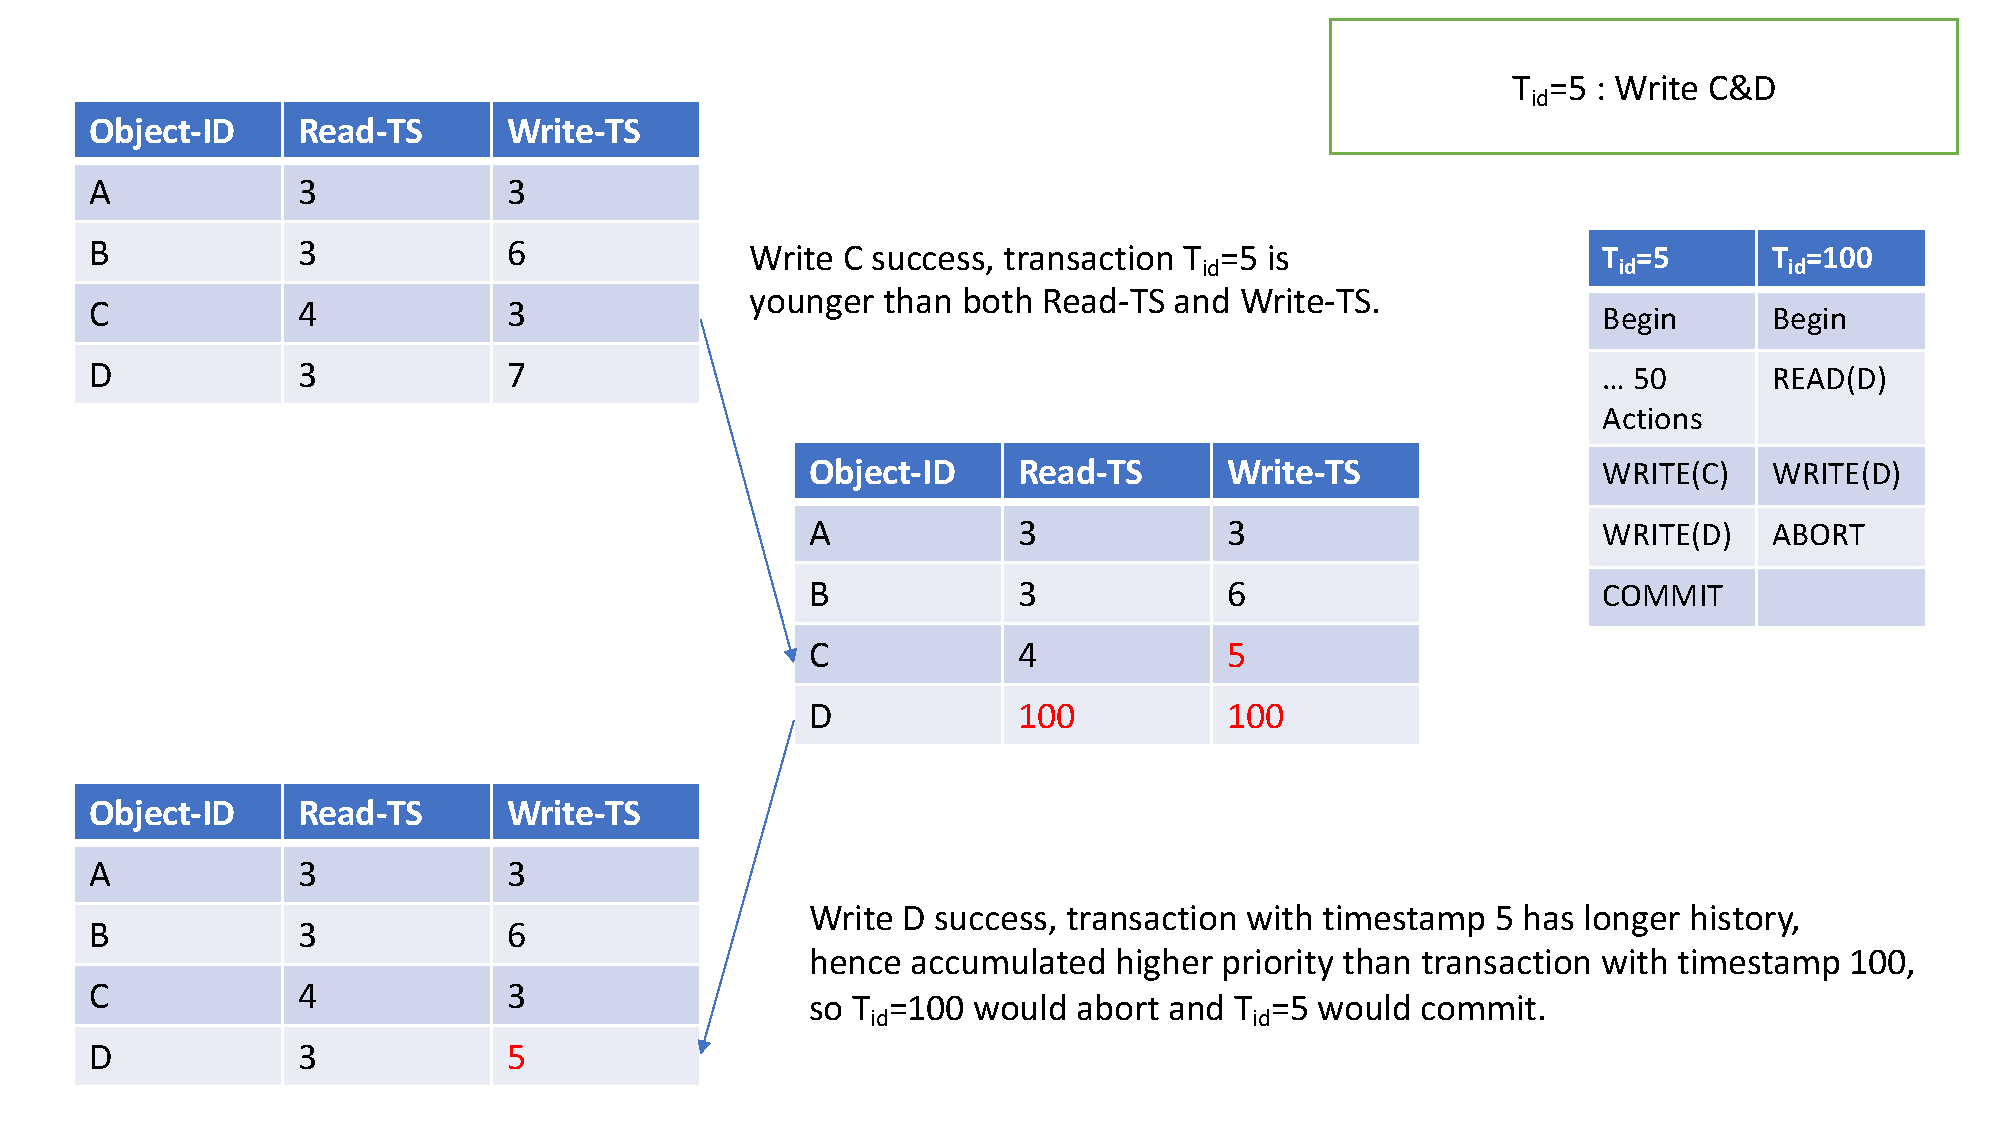
\includegraphics[width=0.9\linewidth]{ourTO.pdf}
	\caption{Our Modifications on Timestamp Ordering}
\end{figure}

The idea of this scheme is the cost of computations for each transaction is sunk after commit or abort, so with the same cost, as many work being done as better, which means aborting short lived (young) transaction is better than abort long lived (old) transaction. The priority of each transaction could be cumulatively which means it is determined by how many actions this transaction has done with each read or write considered as one action. 

The priority can also being determined by the transaction pattern. Since transactions are often used to conduct a complex combination of acts in order to achieve a higher level function, they can have different pattern in terms of read/write order. For example, in the case of banking transaction, inter-bank transaction and single-bank transaction could have different order on read and write to certain object. And we could consider inter-bank transactions have higher priority than single bank transactions, then we could determine the transaction pattern for those two different types of transactions. So whenever a transaction is classified as inter-bank transaction, and it's competing transaction is single bank transaction, the prior would have higher priority to commit which reduces a lot of time on re-do the inter-bank transactions potentially involve more actions and higher requirements on integrity between banks.

\section{Conclusion}

Throughout this survey, we have learned and discussed major concurrency control protocols in modern database systems. And it is clear that in modern database systems, Multi-Version Concurrency Control holds the significant place, since it is the most applied concurrency control protocol, and it has many variants as well as corporation with other concurrency control protocols.

Two-Phase lock is another widely applied concurrency control, it is the symbol of pessimistic protocol, using two phases to lock resources and release locks, it resolves contention but also introduce high overhead on locking mechanism. It is very useful when applied with MVCC since it can handle the write-write contention where MVCC lacks the capability.

Timestamp ordering could be seen as the origin for most modern concurrency control protocols, MVCC originated from MVTO, and Optimistic Concurrency Control is also a subcategory of timestamp ordering. Despite the basic timestamp ordering is not very popular and useful, it's variants are still being developed and have very good performance in today's databases.

Optimistic Concurrency Control is also a highly efficient variant of Timestamp Ordering, it introduces the three-phase concurrency control scheme which is later used on many improvements to TO. Being optimistic in contention let it free of locks which considerably reduce the overhead and time consumption.

With the hardware improvements, these algorithms are also further improved, and the most recent development like Tictoc has greatly improved those protocols by increasing parallel threads while reducing abort rate, which greatly improve the performance in terms of throughput of transactions. This algorithm also provide us with new idea on timestamp generating, by avoiding the isolation level of transaction using timestamp assigned to each data record.

And finally, we have made our own modifications based on the knowledge we learned, to further modify the timestamp ordering. On paper, we considered setting priority to each transaction which is determined either by accumulative action numbers or by pre-defined transaction patterns. And based on the priority, the database should then decide which transaction to be aborted within in a contention. Our design is to minimize the waste and do as many actions as possible when a contention happens.

Overall, we have done a lot of reading and learning to investigate this crucial topic in database systems, and we have learned the details about modern databases' concurrency control, we also have learned about the improvements people have done to adapt old protocols when hardware are getting more powerful. We believe it is still a research worthy topic and the result could be applied to not only database systems design but also other major systems where concurrency matters.

\section{Further Improvement}


\bibliography{reference}


\end{document}